% Phase 2 report (#81). Each section lives in sections/<name>.tex and is written
% by its owner (see the section issues); this file only sets up the template,
% the order and the bibliography.
% Build from this folder: `tectonic main.tex`, or pdflatex + bibtex (e.g. Overleaf).
%
% Until every section has landed, a missing section file prints a visible
% placeholder instead of breaking the build, so each owner can build with only
% their own file. The final build must show no placeholder (see README.md).

\documentclass[conference]{IEEEtran}

\usepackage{iftex}
\ifXeTeX
  % Tectonic and xelatex: Times-like text to match pdflatex's IEEEtran output.
  \usepackage{fontspec}
  \defaultfontfeatures{Extension=.otf, UprightFont=*-regular, BoldFont=*-bold,
    ItalicFont=*-italic, BoldItalicFont=*-bolditalic}
  \setmainfont{texgyretermes}
  \setsansfont{texgyreheros}
  \setmonofont{texgyrecursor}
\fi
\usepackage{cite}
\usepackage{amsmath,amssymb}
\usepackage{graphicx}
\usepackage{url}
\usepackage{tikz}
\usetikzlibrary{arrows.meta,positioning}

% \sectionfile{file}{heading}{issue}: input sections/<file>.tex if it exists,
% otherwise a placeholder section that names the issue still to deliver it.
\newcommand{\sectionfile}[3]{%
  \IfFileExists{sections/#1.tex}{\input{sections/#1}}{%
    \section{#2}\textbf{[Placeholder: \texttt{\detokenize{sections/#1.tex}}, issue~\##3.]}}}

% Bibliography: refs.bib once #80 consolidates it; until then the Phase 1
% references plus every section fragment that exists.
\def\bibfiles{../phase1/refs}
\newcommand{\addbib}[1]{\IfFileExists{sections/#1.bib}{\edef\bibfiles{\bibfiles,sections/#1}}{}}
\addbib{dl_dataset}\addbib{literature_review}\addbib{theory}
\addbib{ablations}\addbib{validation}\addbib{interpretability}

\begin{document}

\title{Sequence and Hybrid Deep Models for\\
Remaining Useful Life Prediction on C-MAPSS:\\
Phase 2}

\author{\IEEEauthorblockN{Gokul VKS, Milind Bansal, Isha Tomar, Yashi Agrawal and Mohammad Affan Anas}
\IEEEauthorblockA{Newton School of Technology, Rishihood University\\
Code and results: \url{https://github.com/vks-g/cmapss-rul-hybrid}}}

\maketitle

\IfFileExists{sections/abstract.tex}{% Abstract and index terms (#81, part "Abstract and introduction"; owner: 11yashiagrawal).
% Cross-validation numbers: results/metrics/fd001_rul_cap_choice.json (#55),
% fd001_ml_capped_cv.json (#61), fd001_cv_{lstm,tcn,transformer}{,_uncapped}.json,
% fd001_hybrid_value_test.json (#68). Official-test numbers arrive with #71:
% every \pending{} must be replaced before the final build.

\providecommand{\pending}[1]{\textbf{[#1]}\typeout{Placeholder: pending #1}}

\begin{abstract}
Remaining useful life (RUL) prediction estimates how many cycles an engine has
left before it fails. Phase~1 of this project built feature-based
machine-learning baselines on the NASA C-MAPSS subset FD001. Phase~2 asks
whether deep models that read the raw sensor sequence do better under the same
leakage-controlled protocol. We first choose the training cap from the
training engines alone: a health index, a hinge fit per engine and the 90th
percentile of the onset RUL rule out caps of 150 and no cap, and support 125.
We then compare an LSTM, a temporal convolutional network and a Transformer,
which share one encoder--head contract, with Random Forest, XGBoost and
Elastic Net retuned on the same capped target and selection metric, and with
two hybrids that fuse a sequence encoder with engineered features. In
engine-grouped cross-validation, the training target matters far more than the
architecture: removing the cap costs every deep encoder 13 to 15 cycles of
RMSE, while the three encoders lie within 1.7 cycles of each other (15.6 to
17.2). The LSTM and Transformer beat machine learning on raw sensors by about
three cycles, but XGBoost on the Phase~1 engineered features remains best (14.5).
Neither hybrid beats its best single branch on accuracy under a test fixed in
advance; gated fusion only lowers the variance across seeds. On the 100
official test engines, scored once after the model freeze,
\pending{\#71: final test RMSE and NASA score of the frozen models}.
\end{abstract}

\begin{IEEEkeywords}
remaining useful life, predictive maintenance, C-MAPSS, LSTM, temporal
convolutional network, Transformer, hybrid models, evaluation protocol
\end{IEEEkeywords}
}{%
  \begin{abstract}\textbf{[Placeholder: \texttt{sections/abstract.tex}, issue~\#81.]}\end{abstract}}

\sectionfile{introduction}{Introduction}{81}
\sectionfile{literature_review}{Deep Learning on C-MAPSS}{63}

% target.tex (#55) is a subsection, so it gets its parent heading here.
\section{Training Target and Model Selection}
\label{sec:target_selection}
\IfFileExists{sections/target.tex}{% Input from reports/phase2/ with amsmath,
% graphicx and cite loaded. Numbers come from scripts/choose_rul_cap.py
% (results/metrics/fd001_rul_cap_*.{json,csv}); figures from
% notebooks/phase2/05_rul_cap.ipynb. Cites Phase 1 keys in reports/phase1/refs.bib.

\subsection{Choosing the RUL Cap}
\label{sec:target}

A training engine in C-MAPSS runs until failure~\cite{Saxena2008damage},
so its uncapped RUL early in life can exceed 300 cycles. While the engine is
healthy its sensors are flat, so an engine with 300 cycles left cannot be told
apart from one with 200. The usual remedy is a piecewise-linear target,
$\min(y_{u,t},c)$, which is flat at a cap $c$ and then falls to
zero~\cite{Heimes2008recurrent}. Phase~1 used $c=125$ from the literature.
Here the cap is chosen with a rule that opens only \texttt{train\_FD001.txt}.

\paragraph{Health index and onset.}
Inside each training fold, the sensors retained by the variance check and
correlated with the cycles to failure ($|r|\geq0.1$; 15 on FD001) are
z-scored with the fold's statistics. Each one is multiplied by the sign of
that correlation, so that all of them rise toward failure, and the results
are averaged into one health index $h_{u,t}$. For every engine a hinge
\begin{equation}
 h_{u,t}\approx a_u+b_u\max(t-\tau_u,0),\qquad b_u>0,
\end{equation}
is fitted by least squares over every candidate bend $\tau_u$ that leaves at
least five cycles on each side. The onset RUL is $T_u-\tau_u$, where $T_u$ is
the failure cycle. On FD001 it has a median of 92 cycles and ranges from 59 to
180 (Fig.~\ref{fig:target_hinge}).

\paragraph{Selection metric.}
$K$ is the 90th percentile of the onset RULs in the training fold. A
candidate cap is scored on held-out engines by
\begin{equation}
 \mathrm{RMSE}_{\leq K}=\sqrt{\frac{1}{|S|}\sum_{(u,t)\in S}(\hat y_{u,t}-y_{u,t})^2},
\end{equation}
with $S=\{(u,t):y_{u,t}\leq K\}$ the held-out cycles at or below $K$, where $y$ is the true, uncapped RUL. Cycles above $K$ are dropped because, for
nine engines in ten, no degradation is visible there yet, and the official
test engines (cut off before failure) rarely reach those values. Scoring
every held-out cycle would instead prefer no cap, because a capped model
necessarily misses training cycles with RUL above 200
(Table~\ref{tab:target_caps}). The metric is \texttt{rul.data.target.selection\_rmse}
and is shared by all later tuning and ablations.

\paragraph{Results.}
Five split seeds (3 engine-grouped folds each) gave $K$ between 123 and
137 (mean 130). The seed-42 folds give 134, 132 and 123, which matches the
prototype. Random Forest, XGBoost~\cite{Chen2016xgboost} and Elastic
Net~\cite{Zou2005regularization} were retrained with the Phase~1 engineered
features and hyperparameters at caps of 100, 125, 150 and none.
Caps of 150 and none are clearly worse on $\mathrm{RMSE}_{\leq K}$, by 2.5 to
15 cycles. Caps of 100 and 125 are close. Random Forest picks 125 on all five
seeds and XGBoost on four of five (by 0.04 cycles), while Elastic Net picks 100 on all five.
Averaged over the three models, the two caps tie (16.38 vs.\ 16.40).

\begin{table}[t]
\centering
\caption{FD001 held-out RMSE by training cap (mean $\pm$ s.d.\ over five seeds of
the 3-fold mean). ``All'': every held-out cycle. ``$\leq K$'': the selection metric.}
\label{tab:target_caps}
\footnotesize
\setlength{\tabcolsep}{2.5pt}
\begin{tabular}{lcccc}
\hline
Model, metric & 100 & 125 & 150 & none \\
\hline
RF, all & 58.33$\pm$0.21 & 47.94$\pm$0.09 & 41.22$\pm$0.24 & \textbf{36.73}$\pm$0.55 \\
RF, $\leq K$ & 15.62$\pm$0.36 & \textbf{14.97}$\pm$0.30 & 17.42$\pm$0.36 & 23.57$\pm$0.70 \\
XGB, $\leq K$ & 15.57$\pm$0.38 & \textbf{15.54}$\pm$0.38 & 18.19$\pm$0.26 & 24.97$\pm$0.89 \\
EN, $\leq K$ & \textbf{17.94}$\pm$0.14 & 18.68$\pm$0.18 & 22.87$\pm$0.31 & 32.69$\pm$0.73 \\
\hline
\end{tabular}
\end{table}

\paragraph{Sensitivity.}
The choice between 100 and 125 depends on the percentile. With the 85th
percentile or lower ($K\leq117$), all 15 seed--model runs pick 100. With the
95th ($K\approx141$), all 15 pick 125. The 90th percentile lies on the
boundary (9 of 15 runs pick 125). This agrees with the prototype, where
$K\approx106$ selected 100.

\paragraph{Decision and caveats.}
The rule rules out 150 and an uncapped target, but it cannot separate 100
from 125. We keep $c=125$. The strongest Phase~1 model prefers it on every
seed, and the other Phase~2 results already use it, so switching would cost a
full retrain for no measurable gain. Four caveats apply. (i)~The official test
RMSE at $c=125$ (16.21) was known before this rule was designed, so this
section shows that 125 is defensible from training data alone; it is not a
blind choice. (ii)~Only the tabular models were rerun; the sequence models
may prefer a different cap. (iii)~Hyperparameters were not retuned per cap.
(iv)~The hinge assumes a single bend, and noisy engines can stretch the
upper tail of the onset distribution, which is where $K$ is read.

\begin{figure}[t]
\centering
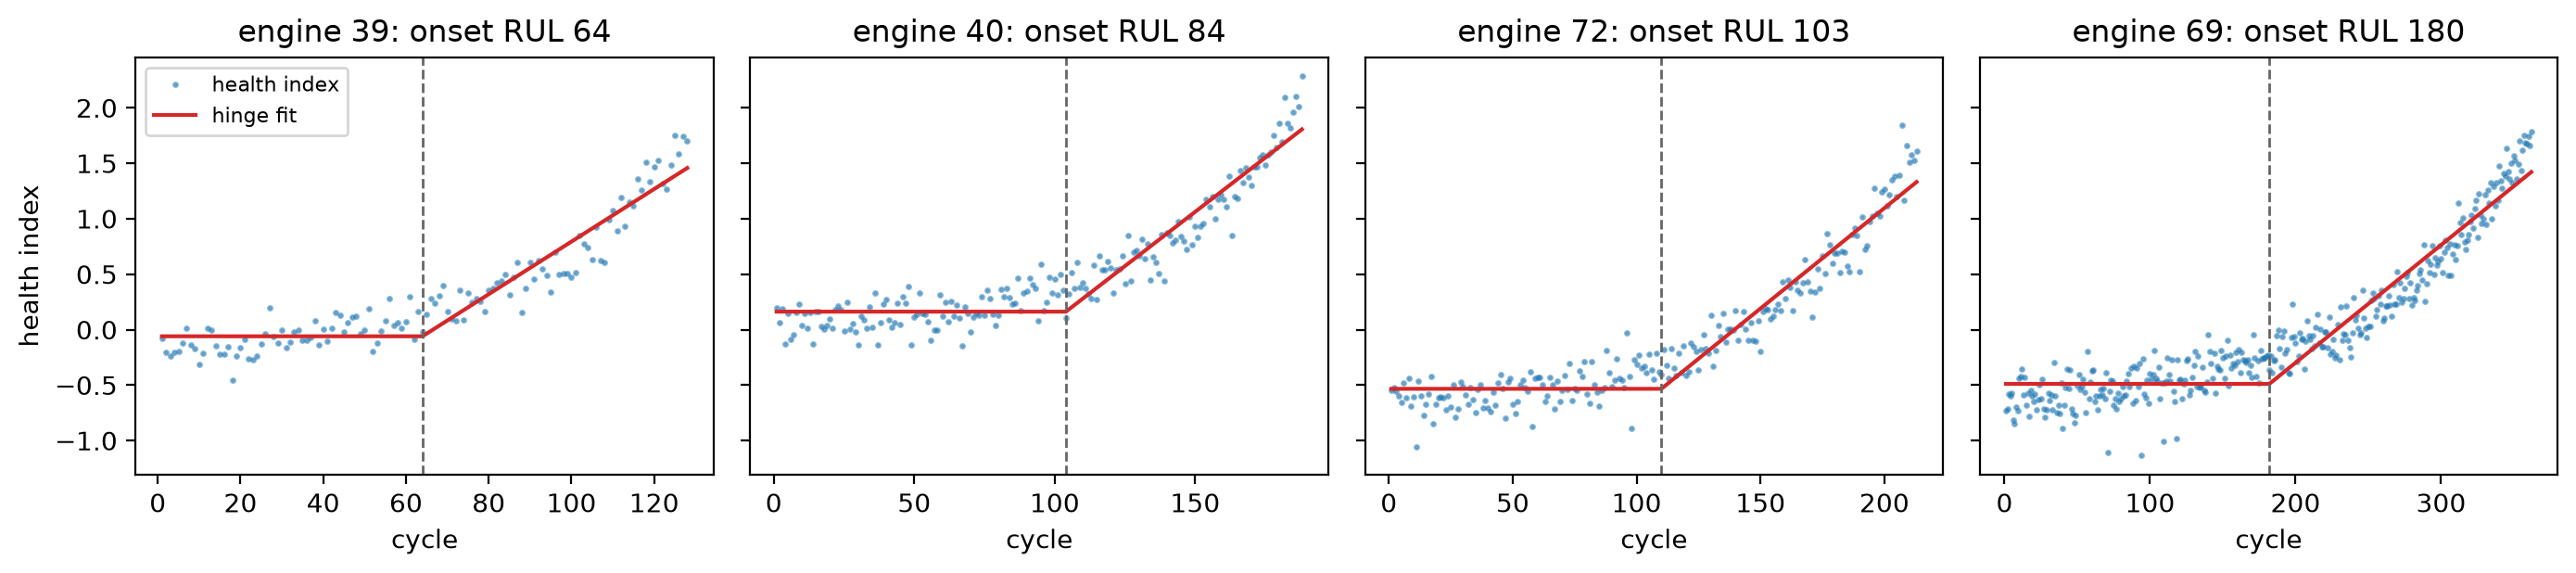
\includegraphics[width=\linewidth]{../../results/figures/fd001_rul_cap_hinge_fits.png}\\[2pt]
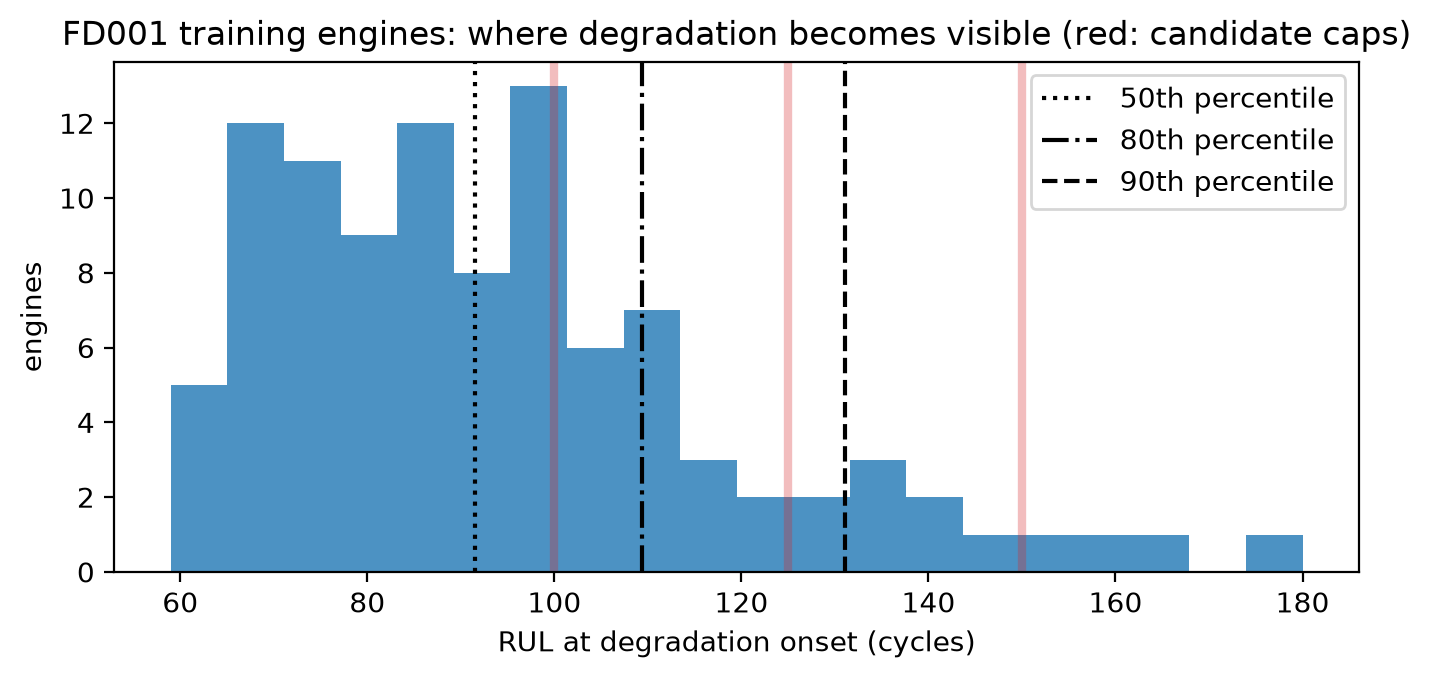
\includegraphics[width=0.49\linewidth]{../../results/figures/fd001_rul_cap_onset_distribution.png}\hfill
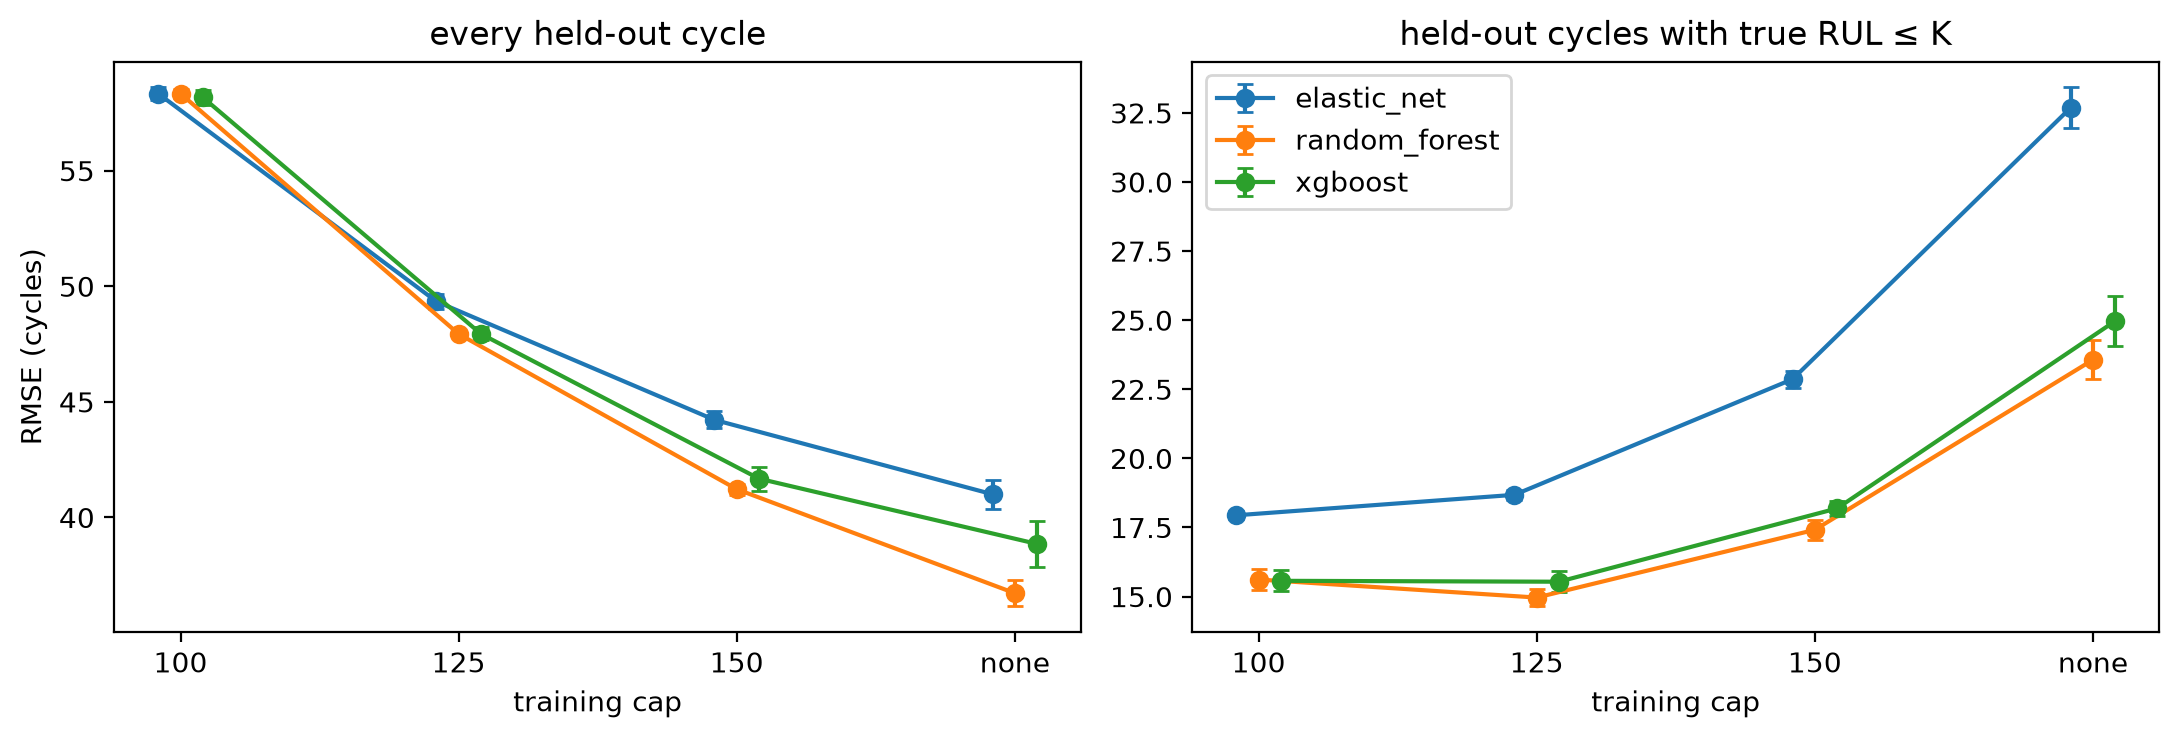
\includegraphics[width=0.49\linewidth]{../../results/figures/fd001_rul_cap_score_by_cap.png}
\caption{Top: hinge fits for four FD001 training engines. Bottom left: onset RUL
distribution, with candidate caps in red. Bottom right: held-out RMSE by cap,
on every cycle and on cycles with true RUL $\leq K$.}
\label{fig:target_hinge}
\end{figure}
}{%
  \textbf{[Placeholder: \texttt{sections/target.tex}, issue~\#55.]}}

\sectionfile{dl_dataset}{Sequence Dataset and Regularization}{74}
\sectionfile{theory}{Theory of the Phase 2 Models}{67}
\sectionfile{architecture}{Model Architectures}{81}
\sectionfile{hybrid}{Hybrid Architectures}{81}
\sectionfile{ablations}{Ablation Studies}{75}
\sectionfile{validation}{Technical Validation}{76}
\sectionfile{interpretability}{Interpretability}{76}
\sectionfile{results}{Results and Discussion}{81}
\sectionfile{conclusion}{Conclusion and Future Work}{81}
\sectionfile{contributions}{Author Contributions}{81}

\bibliographystyle{IEEEtran}
\IfFileExists{refs.bib}{\bibliography{refs}}{\bibliography{\bibfiles}}

\end{document}
